\documentclass[11pt]{report}
\title{Assignment 2: Coin Counter}
\author{Guilherme Santos \texttt{fc62533}}
\date{\today}

\usepackage[left=1in,right=1in,top=1in,bottom=1in]{geometry}
\usepackage{tikz,pgfplots}
\usepackage{subfig}
\usepackage{caption}
\usepackage{amsmath}
\begin{document}

\maketitle

\noindent The strategy used was the Fork/Join framework because the algorithm provided is recursive, 
so it is possible to divide the set of coins into smaller parts and create sub-tasks to compute those same parts.
Regarding the granularity of the task, I tested the execution times with \texttt{index $\ge$ 15} and \texttt{getQueuedTaskCount() $>$ 2} and was able to conclude that with \texttt{index $\ge$ 15} the execution is faster. 
The best result I got was $\approx$ 0.082 seconds with 24 threads.

\begin{figure}[h]
  
    \caption*{Execution time of each iteration with \texttt{coins.length=30} and \texttt{LIMIT=999}}
   
    \begin{minipage}{0.5\textwidth}
      \centering
      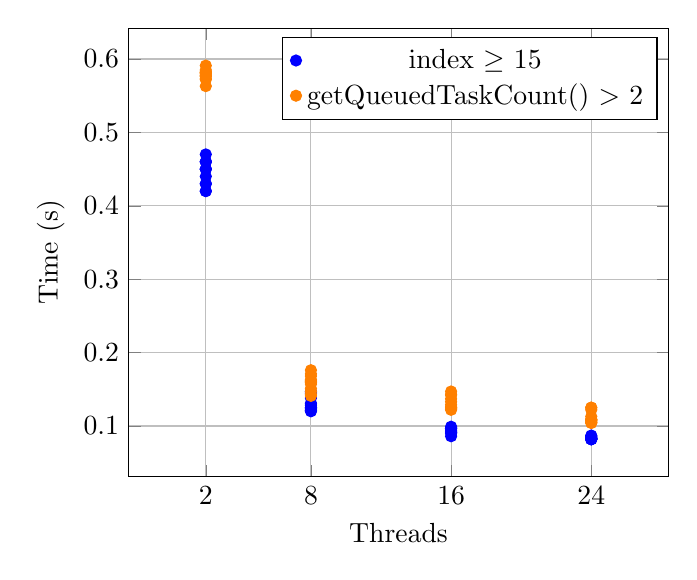
\begin{tikzpicture}
        \begin{axis}[grid=major, xlabel={Threads}, ylabel={Time (s)}, ytick={0.6,0.5,...,0.1}, xtick={2, 8, 16, 24},xtick={2, 8, 16, 24}, enlarge x limits=0.2]
          \addplot+[only marks, mark size=2pt, mark options={mark=*, blue}]
          coordinates {
            (2,0.45)
            (2,0.44)
            (2,0.46)
            (2,0.42)
            (2,0.43)
            (2,0.47)
            (2,0.46)
            (2,0.42)
            (2,0.43)
            (2,0.46)
            (2,0.45)
            (2,0.45)
            (8,0.121)
            (8,0.147)
            (8,0.130)
            (8,0.121)
            (8,0.128)
            (8,0.138)
            (8,0.124)
            (8,0.120)
            (8,0.146)
            (8,0.144)
            (8,0.131)
            (8,0.125)
            (8,0.125)
            (8,0.122)
            (16,0.092)
            (16,0.094)
            (16,0.099)
            (16,0.097)
            (16,0.091)
            (16,0.090)
            (16,0.086)
            (16,0.097)
            (16,0.091)
            (16,0.096)
            (16,0.092)
            (16,0.097)
            (24,0.086) 
            (24,0.082) 
            (24,0.082) 
            (24,0.083) 
            (24,0.082)
            (24,0.082) 
            (24,0.085) 
            (24,0.087) 
            (24,0.084) 
            (24,0.082)
            (24,0.083) 
            (24,0.083)
          };
          \addlegendentry{index $\ge$ 15}; % Label for the first group

      \addplot+[only marks, mark size=2pt, mark options={mark=*, orange}]
        coordinates {
          (2,0.576)
          (2,0.582)
          (2,0.573)
          (2,0.577)
          (2,0.580)
          (2,0.581)
          (2,0.563)
          (2,0.572)
          (2,0.582)
          (2,0.585)
          (2,0.578)
          (2,0.591)
          (8,0.168)
          (8,0.147)
          (8,0.176)
          (8,0.161)
          (8,0.163)
          (8,0.141)
          (8,0.151)
          (8,0.143)
          (8,0.160)
          (8,0.159)
          (8,0.157)
          (8,0.171)
          (8,0.162)
          (8,0.160)
          (16,0.122)
          (16,0.142)
          (16,0.143)
          (16,0.125)
          (16,0.125)
          (16,0.129)
          (16,0.147)
          (16,0.124)
          (16,0.133)
          (16,0.137)
          (16,0.126)
          (16,0.123)
          (24,0.125) 
          (24,0.109) 
          (24,0.113) 
          (24,0.105) 
          (24,0.125)
          (24,0.122) 
          (24,0.105) 
          (24,0.107) 
          (24,0.108) 
          (24,0.104)
          (24,0.109) 
          (24,0.108)
    };
    \addlegendentry{getQueuedTaskCount() $>$ 2}; % Label for the second group
        \end{axis}
      \end{tikzpicture}
      
      \caption{Parallel}
    \end{minipage}%
    \hspace{2em}
    \begin{minipage}{0.5\textwidth}
      \centering
      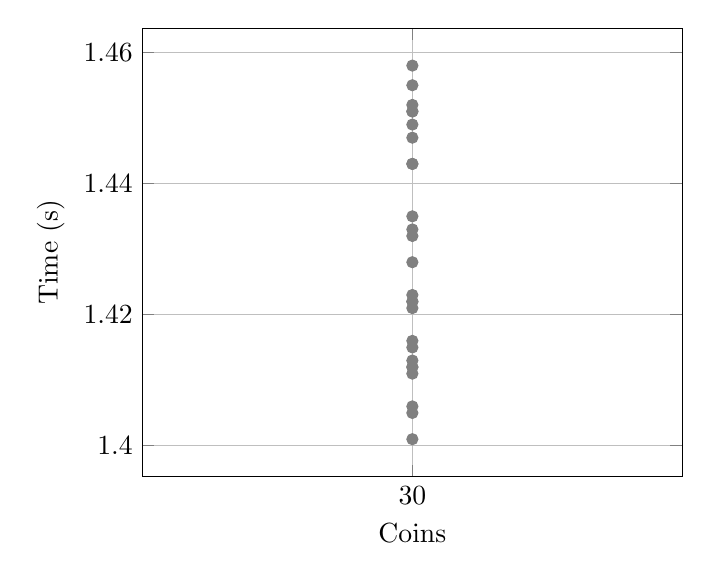
\begin{tikzpicture}
        \begin{axis}[grid=major, xlabel={Coins}, ylabel={Time (s)}, xtick={30}]
          \addplot+[only marks, mark size=2pt, mark options={mark=*, gray}]
          coordinates {
            (30,1.455)
            (30,1.406)
            (30,1.405)
            (30,1.401)
            (30,1.411)
            (30,1.412)
            (30,1.413)
            (30,1.428)
            (30,1.443)
            (30,1.447)
            (30,1.451)
            (30,1.432)
            (30,1.433)
            (30,1.435)
            (30,1.458)
            (30,1.423)
            (30,1.422)
            (30,1.422)
            (30,1.415)
            (30,1.416)
            (30,1.412)
            (30,1.421)
            (30,1.449)
            (30,1.443)
            (30,1.452)
            (30,1.451)
          };
        \end{axis}
      \end{tikzpicture}
      \caption{Sequential}
    \end{minipage}
\end{figure}

$$SpeedUp = \frac{\overline{Sequential}}{\overline{Parallel}} = \frac{1.44s}{0.085s} \approx 17 $$
$$Occupancy = \frac{{Speedup}}{\#Cores} = \frac{17}{24} \approx 0.71 $$

\section*{Hardware details}
\begin{tabular}{|c|c|c|c|c|c|}
  \hline
  CPU & Cores & Threads & RAM &  Operating System & Java\\
  \hline
  Intel Core i7-13700 & 16 & 24 & 32GB 6000MHz & Windows 11 & 21\\
  \hline
\end{tabular}

\end{document}